% This file was created with tikzplotlib v0.10.1.
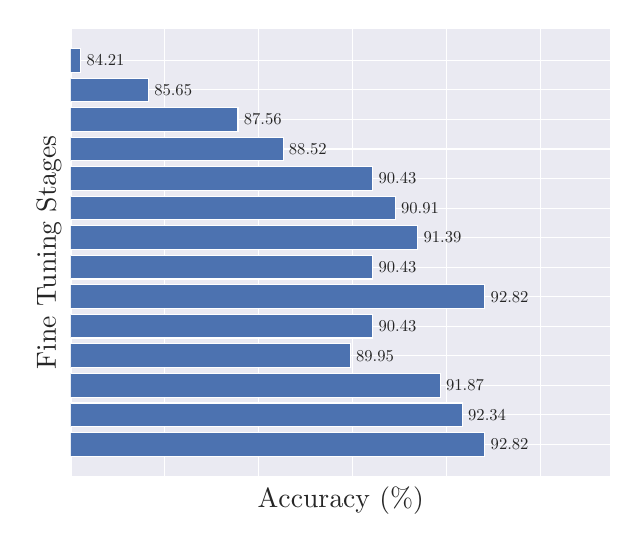
\begin{tikzpicture}

\definecolor{darkslategray38}{RGB}{38,38,38}
\definecolor{lavender234234242}{RGB}{234,234,242}
\definecolor{steelblue76114176}{RGB}{76,114,176}

\begin{axis}[
axis background/.style={fill=lavender234234242},
axis line style={white},
tick align=outside,
x grid style={white},
xlabel=\textcolor{darkslategray38}{Accuracy (\%)},
xmajorgrids,
xmajorticks=false,
xmin=84, xmax=95.5,
xtick style={color=darkslategray38},
y grid style={white},
ylabel=\textcolor{darkslategray38}{Fine Tuning Stages},
ymajorgrids,
ymajorticks=false,
ymin=-1.09, ymax=14.09,
ytick style={color=darkslategray38},
ytick={0,1,2,3,4,5,6,7,8,9,10,11,12,13},
yticklabels={
  13th Stage,
  12th Stage,
  11th Stage,
  10th Stage,
  9th Stage,
  8th Stage,
  7th Stage,
  6th Stage,
  5th Stage,
  4th Stage,
  3rd Stage,
  2nd Stage,
  1st Stage,
  Base Line
}
]
\draw[draw=white,fill=steelblue76114176] (axis cs:0,-0.4) rectangle (axis cs:92.82,0.4);
\draw[draw=white,fill=steelblue76114176] (axis cs:0,0.6) rectangle (axis cs:92.34,1.4);
\draw[draw=white,fill=steelblue76114176] (axis cs:0,1.6) rectangle (axis cs:91.87,2.4);
\draw[draw=white,fill=steelblue76114176] (axis cs:0,2.6) rectangle (axis cs:89.95,3.4);
\draw[draw=white,fill=steelblue76114176] (axis cs:0,3.6) rectangle (axis cs:90.43,4.4);
\draw[draw=white,fill=steelblue76114176] (axis cs:0,4.6) rectangle (axis cs:92.82,5.4);
\draw[draw=white,fill=steelblue76114176] (axis cs:0,5.6) rectangle (axis cs:90.43,6.4);
\draw[draw=white,fill=steelblue76114176] (axis cs:0,6.6) rectangle (axis cs:91.39,7.4);
\draw[draw=white,fill=steelblue76114176] (axis cs:0,7.6) rectangle (axis cs:90.91,8.4);
\draw[draw=white,fill=steelblue76114176] (axis cs:0,8.6) rectangle (axis cs:90.43,9.4);
\draw[draw=white,fill=steelblue76114176] (axis cs:0,9.6) rectangle (axis cs:88.52,10.4);
\draw[draw=white,fill=steelblue76114176] (axis cs:0,10.6) rectangle (axis cs:87.56,11.4);
\draw[draw=white,fill=steelblue76114176] (axis cs:0,11.6) rectangle (axis cs:85.65,12.4);
\draw[draw=white,fill=steelblue76114176] (axis cs:0,12.6) rectangle (axis cs:84.21,13.4);
\draw (axis cs:92.82,0) ++(0pt,0pt) node[
  scale=0.6,
  anchor=west,
  text=darkslategray38,
  rotate=0.0
]{92.82};
\draw (axis cs:92.34,1) ++(0pt,0pt) node[
  scale=0.6,
  anchor=west,
  text=darkslategray38,
  rotate=0.0
]{92.34};
\draw (axis cs:91.87,2) ++(0pt,0pt) node[
  scale=0.6,
  anchor=west,
  text=darkslategray38,
  rotate=0.0
]{91.87};
\draw (axis cs:89.95,3) ++(0pt,0pt) node[
  scale=0.6,
  anchor=west,
  text=darkslategray38,
  rotate=0.0
]{89.95};
\draw (axis cs:90.43,4) ++(0pt,0pt) node[
  scale=0.6,
  anchor=west,
  text=darkslategray38,
  rotate=0.0
]{90.43};
\draw (axis cs:92.82,5) ++(0pt,0pt) node[
  scale=0.6,
  anchor=west,
  text=darkslategray38,
  rotate=0.0
]{92.82};
\draw (axis cs:90.43,6) ++(0pt,0pt) node[
  scale=0.6,
  anchor=west,
  text=darkslategray38,
  rotate=0.0
]{90.43};
\draw (axis cs:91.39,7) ++(0pt,0pt) node[
  scale=0.6,
  anchor=west,
  text=darkslategray38,
  rotate=0.0
]{91.39};
\draw (axis cs:90.91,8) ++(0pt,0pt) node[
  scale=0.6,
  anchor=west,
  text=darkslategray38,
  rotate=0.0
]{90.91};
\draw (axis cs:90.43,9) ++(0pt,0pt) node[
  scale=0.6,
  anchor=west,
  text=darkslategray38,
  rotate=0.0
]{90.43};
\draw (axis cs:88.52,10) ++(0pt,0pt) node[
  scale=0.6,
  anchor=west,
  text=darkslategray38,
  rotate=0.0
]{88.52};
\draw (axis cs:87.56,11) ++(0pt,0pt) node[
  scale=0.6,
  anchor=west,
  text=darkslategray38,
  rotate=0.0
]{87.56};
\draw (axis cs:85.65,12) ++(0pt,0pt) node[
  scale=0.6,
  anchor=west,
  text=darkslategray38,
  rotate=0.0
]{85.65};
\draw (axis cs:84.21,13) ++(0pt,0pt) node[
  scale=0.6,
  anchor=west,
  text=darkslategray38,
  rotate=0.0
]{84.21};
\end{axis}

\end{tikzpicture}
